%\documentclass[11pt, twoside, b5paper]{book}
\documentclass[11pt, twoside, b5paper]{extbook}

\usepackage[b5paper, margin=2cm, innermargin=2cm]{geometry}
%\usepackage[b5paper]{geometry}
%\geometry{verbose, tmargin=1.9cm, bmargin=1.9cm, lmargin=1.9cm, rmargin=1.2cm}

%\usepackage{bera}
\usepackage{fancyhdr}
%\usepackage[Bjornstrup]{fncychap}

\pagestyle{plain}

\usepackage{emptypage}
\usepackage{subfiles}
\usepackage{color}
\definecolor{mygray}{gray}{0.75}
\definecolor{dkblue}{rgb}{0,0,0.4}
\usepackage[table]{xcolor}

\usepackage{imakeidx}
\usepackage{hyperref}
\makeindex[name=authors,title=Authors,intoc=true]
\hypersetup{pdftitle={IPMU 2020 Book of abstracts},
 pdfauthor={Fernando Batista},
 pdfsubject={IPMU 2020},
 pdfkeywords={IPMU 2020, book of abstracts},
 colorlinks, citecolor=dkblue, filecolor=dkblue, linkcolor=dkblue, urlcolor=blue}

\usepackage[utf8]{inputenc}
\usepackage[T1]{fontenc}

\usepackage{eurosym}
\usepackage{amsfonts, amsmath, hanging, parskip, times}
\usepackage[numbers]{natbib}
\usepackage[pdftex]{graphicx}
\usepackage{wrapfig}

\usepackage{pdfpages}

\newcommand\keywords[1]{%
    \begingroup
    \def\and{-- }
    \par
    \noindent\textbf{Keywords: } #1\par
    \endgroup
}

\providecommand{\tightlist}{%
	\setlength{\itemsep}{0pt}\setlength{\parskip}{0pt}}

% Table of Contents format
\usepackage{tocloft}
\cftsetindents{section}{1em}{2em}
\cftsetindents{subsection}{2em}{1em}
\renewcommand\cftchapfont{\sffamily\bfseries}
\renewcommand\cftsecfont{\bfseries}
%\renewcommand\cftchapafterpnum{\par\addvspace{4pt}}
\renewcommand\cftsecafterpnum{\par\addvspace{3pt}}
\setlength{\cftbeforesecskip}{6pt}

\setcounter{secnumdepth}{0}
\setcounter{tocdepth}{2}

% Chapter and section formats 
\usepackage{titlesec}

%\titleformat{\chapter}[display]{\normalfont\huge\bfseries}{\chaptertitlename\ \thechapter}{20pt}{\Huge}   
%\titlespacing*{\chapter}{0pt}{-50pt}{40pt}
% \titleformat{\chapter}[display]{\normalfont\bfseries}{}{0pt}{\Large}

%\titleformat{\section}[block]{\Large\bfseries}{}{0pt}{\\}[\vspace{2pt}]
%\titleformat{\section}[block]{\Large\bfseries\filcenter}{}{1em}{}
\titleformat{\subsection}[block]{\Large\bfseries\filcenter}{}{1em}{}

\newcommand{\colorsection}[1]{%
  \colorbox{black!15}{\parbox[c][1.5cm]{\dimexpr\textwidth-2\fboxsep}{\begin{center}#1\end{center}}}}
\titleformat{name=\section}[block]{\sffamily\bfseries\Large}{}{0pt}{\colorsection}  
\newcommand{\mysection}[3]{%
	\hypertarget{#2}{}\section[#1\\ \normalfont \small \textit{#3}]{#1}\label{#2}
	\begin{center}#3\end{center}%
}

\newcommand{\colorchapter}[1]{%
  \colorbox{black!15}{\parbox[b][2.5cm]{\dimexpr\textwidth-2\fboxsep}{\begin{flushright}#1\,\,\,\end{flushright}\vspace{12pt}}}}
\titleformat{name=\chapter}[block]{\sffamily\bfseries\Large}{}{0pt}{\colorchapter}  
%\titlespacing*{\chapter}{0pt}{\baselineskip}{40pt}
\titlespacing*{\chapter}{0pt}{0pt}{40pt}

\newcommand{\mychapter}[1]{
    	\phantomsection
	\chapter*{#1}
	\addcontentsline{toc}{chapter}{#1}
	\markboth{#1}{#1}%
}

\usepackage{ifthen}
\usepackage{array}
\providecommand{\tabularnewline}{\\}

\newenvironment{lyxlist}[1]
	{\begin{list}{}
		{\settowidth{\labelwidth}{#1}
		 \setlength{\leftmargin}{\labelwidth}
		 \addtolength{\leftmargin}{\labelsep}
		 \renewcommand{\makelabel}[1]{##1\hfil}}}
	{\end{list}}
	
\newenvironment{parallelsection}[5]{ % {sessionID}{S1text}{S2text}{S3text}{S4text} 
    \noindent\begin{minipage}[t]{1\columnwidth}%
    \begin{flushright}
    \small%
    \begin{tabular}{|>{\centering}p{0.2\columnwidth}|>{\centering}p{0.2\columnwidth}|>{\centering}p{0.2\columnwidth}|>{\centering}p{0.2\columnwidth}|}
    \hline 
    \cellcolor{blue!10}\hyperlink{#1A}{#2} & 
    \cellcolor{green!10}\hyperlink{#1B}{#3} & 
    \cellcolor{red!10}\hyperlink{#1C}{#4} & 
    \cellcolor{orange!10}\hyperlink{#1D}{#5}\tabularnewline
    \cellcolor{blue!15}\ifthenelse{\equal{#2}{}}{}{\emph{Page~\pageref{#1A}}} &
    \cellcolor{green!15}\ifthenelse{\equal{#3}{}}{}{\emph{Page~\pageref{#1B}}} & 
    \cellcolor{red!15}\ifthenelse{\equal{#4}{}}{}{\emph{Page~\pageref{#1C}}} & 
    \cellcolor{orange!15}\ifthenelse{\equal{#5}{}}{}{\emph{Page~\pageref{#1D}}}\tabularnewline
    \hline
    \end{tabular}
    \par\end{flushright}%
    \end{minipage}
}	
 
 %%%%%%%%%%%%%%%%%%%%%%%%%%%%%%%%%%%%%%%%%%%%%%%%%%%%%%%%
	
\title{\sffamily \textbf{IPMU 2020} \\[1ex]
18th International Conference on Information Processing and Management of Uncertainty in Knowledge-Based Systems}
\author{June 15th – 19th 2020\\[1ex]
{\bf Online Conference} {\em in place of} Lisbon, Portugal}
\date{
{\em Edited by}\\
\vspace{1em}
Joao Paulo Carvalho,
Marek Reformat, 
Marie-Jeanne Lesot,\\
Susana Vieira,
and Fernando Batista\\
\vspace{1em}
ISBN: xxx-xxx-xxxxxx
}

\begin{document}

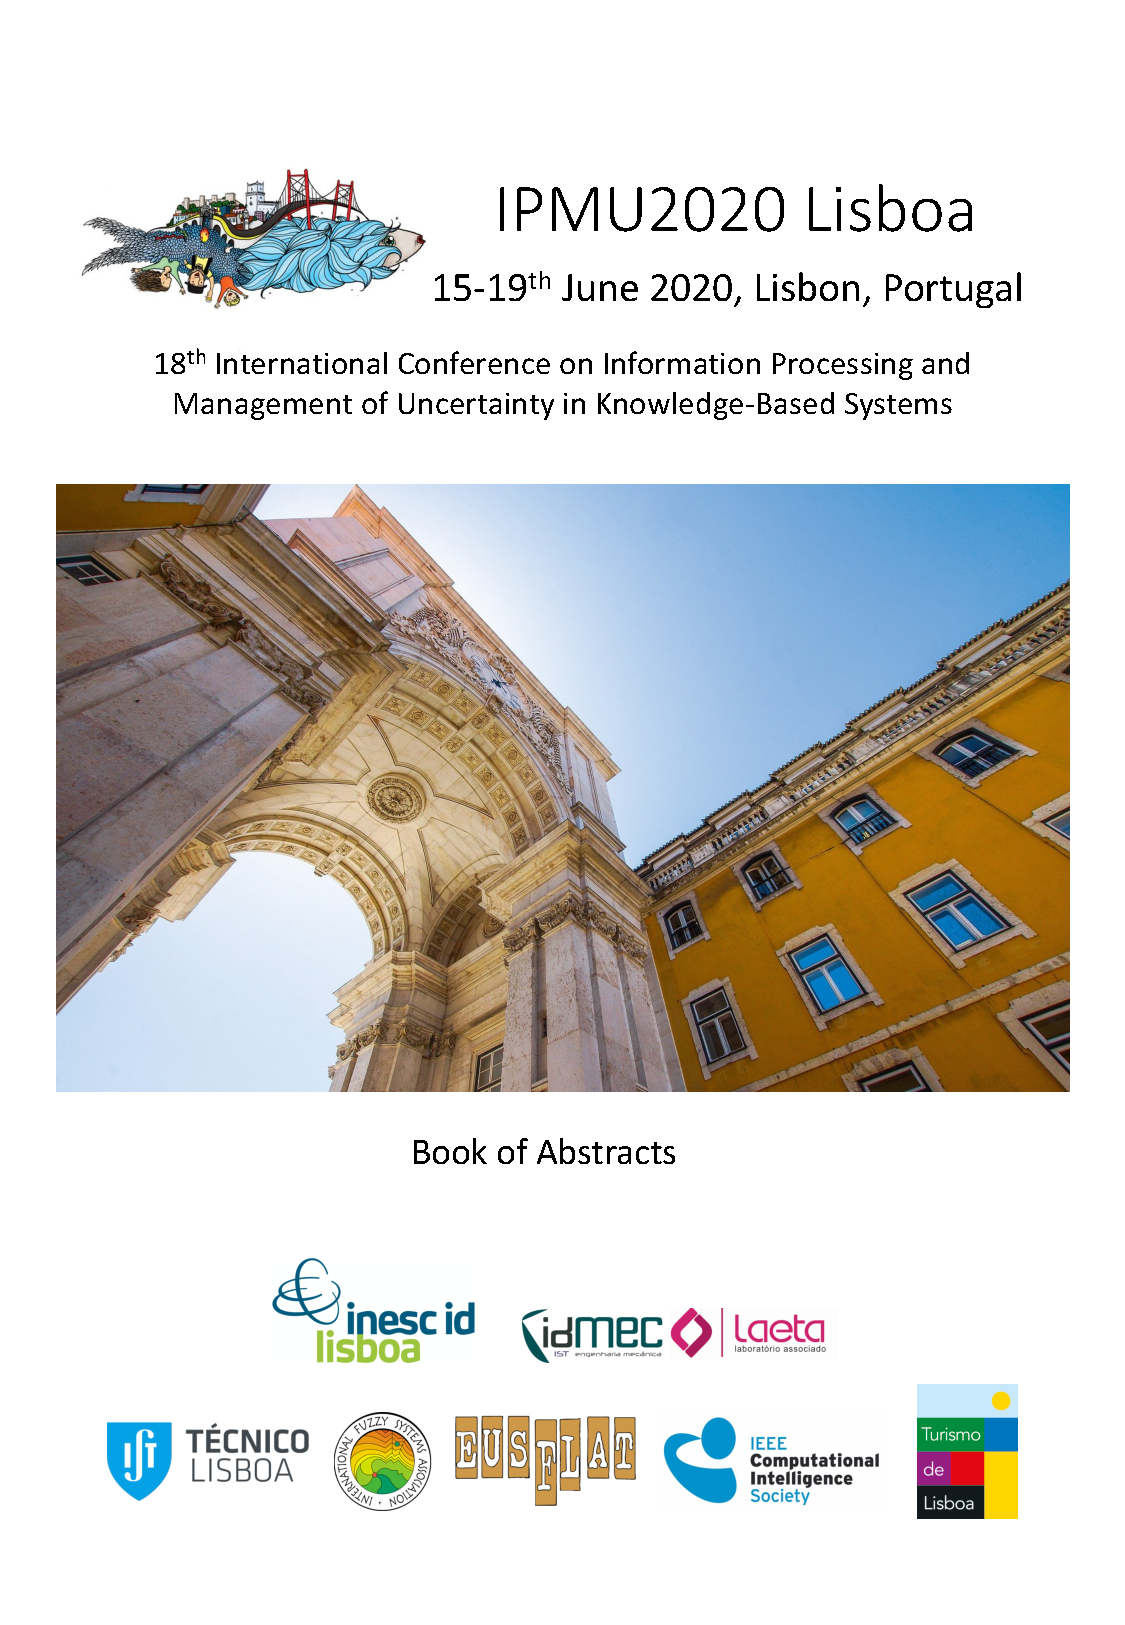
\includepdf{images/front_cover.pdf}
% \cleardoublepage

\clearpage

\frontmatter
\maketitle


\begin{small}
\tableofcontents
\end{small}

\chapter*{The Organizing Committee}

\subsubsection*{General Chair}

Joao Paulo Carvalho (Portugal)

\subsubsection*{Program Chairs}

Marek Reformat (Canada)\\
Marie-Jeanne Lesot (France)\\
Susana Vieira (Portugal)

\subsubsection*{Publication Chair}

Anna Wilbik (Netherlands)

\subsubsection*{Special Session Chair}

Uzay Kaymak (Netherlands)

\subsubsection*{Sponsors and Publicity Chair}

João M. C. Sousa (Portugal)

\subsubsection*{Web Chair}

Fernando Batista (Portugal)

\subsubsection*{Executive directors}

Bernadette BOUCHON-MEUNIER\\
Ronald R. YAGER


\mychapter{Preface} % Welcome to IPMU 2020 
\vspace{5em}

%\input{misc/welcome.tex}
We would like to welcome you to the 18th International Conference on Information Processing and Management of Uncertainty in Knowledge-Based Systems (IPMU 2020). This edition will undoubtedly be marked by the sad fact that, due to the COVID-19 pandemics, it will be the first, and hopefully the last, IPMU conference to be held online.

Under normal circumstances, you would be in beautiful Lisbon, holding this volume in your hands, and looking for overall information regarding the local organization: where will the sessions be, where are the coffee-breaks, what to do in the surroundings, where to grab a coffee, a beer or a nice glass of wine with your friends after the sessions, where will be the Gala dinner... As it is, you are probably reading these lines on a computer screen at your home town, and none of those "not so little things" that bring us all together will be possible. Sad times indeed.

In this document you will find an overview of the IPMU 2020 program, the detailed program organized by sessions, including the respective Session Chairs, the list of the Plenary Talks and respective speakers, and the abstracts of all accepted papers. The document is fully linked in order to easily access the abstracts and facilitate the choice of the sessions to attend.    

The IPMU 2020 conference offers a versatile and comprehensive scientific program: Four invited talks given by distinguished researchers, Barbara Tversky (Stanford University and Columbia University, USA), who will receive the IPMU 2020 Kampé de Fériet Award, Luísa Coheur (INESC-ID / Instituto Superior Técnico, Universidade de Lisboa, Portugal), Jim Keller (University of Missouri, USA), and Björn Schuller (Imperial College London, UK); A special tribute to celebrate the life and achievements of Enrique Ruspini, one of Fuzzy Logic pioneers who passed away last year;  173 papers authored by researchers from 34 different countries distributed by 22 special sessions and several sessions on diverse uncertainty related topics. 


The official webpage of IPMU 2020, \url{https://ipmu2020.inesc-id.pt/}, can be consulted for more information.

Wish you all the best in these difficult times,\\
Hope to see you in Lisbon in the near future,

\vspace{1cm}

\begin{flushleft}
João Paulo Carvalho\\[1ex]
IPMU2020 General-Chair 
\end{flushleft}



\mychapter{Program Overview}

\subsubsection*{Monday, June 15}

\begin{lyxlist}{00:00 -- 00:00}
\item [{15:40 -- 16:00}] \textbf{Opening session}
\item [{16:00 -- 17:00}] \textbf{\emph{Invited Talk: \hyperlink{talk1}{How Action Shapes Thought} (Barbara Tversky)}}
\item [{17:10 -- 18:50}] Parallel Section 1
\end{lyxlist}
\parallelsection{Mo1}{SS2: Theoretical and Applied Aspects of Imprecise Probabilities, part I}{Games \& SS18: Discrete Models and Computational Intelligence}{Real World Applications}{Knowledge Processing and Creation}

\begin{lyxlist}{00:00 -- 00:00}
\item [{19:10~--~20:30}] Parallel Section 2
\end{lyxlist}
\parallelsection{Mo2}{SS2: Theoretical and Applied Aspects of Imprecise Probabilities, part II}{XAI \& SS13: Image Understanding and Explainable AI}{SS10: Fuzzy Implication Functions}{SS11: Soft Methods in Statistics and Data Analysis, part I}

\begin{lyxlist}{00:00 -- 00:00}
\item [{21:00}] Welcome reception BYOD (bring your own drink)
\end{lyxlist}

\vfill
\pagebreak

\subsubsection*{Tuesday, June 16}

\begin{lyxlist}{00:00 -- 00:00}
\item [{14:30 -- 15:30}] Parallel Section 1
\end{lyxlist}
\parallelsection{Tu1}{Image Processing}{SS21: Formal Concept Analysis, Rough Sets, General Operators and Related Topics, part I}{SS9: Computational Intelligence for Logistics and Transportation Problems}{SS11: Soft Methods in Statistics and Data Analysis, part II}

\begin{lyxlist}{00:00 -- 00:00}
\item [{15:40 -- 16:00}] \textbf{Homage to Enrique Ruspini}
\item [{16:00 -- 17:00}] \textbf{\emph{Invited Talk: \hyperlink{talk2}{Average Jane, Where Art Thou? - Recent Avenues in Efficient Machine Learning under Subjectivity Uncertainty} (Björn Schuller)}}
\item [{17:10 -- 18:50}] Parallel Section 2
\end{lyxlist}
\parallelsection{Tu2}{Decision making, preference \& votes}{SS5: Aggregation: Theory and Practice, part I}{SS15: Mathematical Methods Towards Dealing with Uncertainty in Applied Sciences, part I}{SS16: Statistical Image Processing and Analysis, with Applications in Neuroimaging}

\begin{lyxlist}{00:00 -- 00:00}
\item [{17:10 -- 18:50}] Parallel Section 1
\end{lyxlist}
\parallelsection{Tu3}{SS2: Theoretical and Applied Aspects of Imprecise Probabilities, part III}{SS5: Aggregation: Theory and Practice, part II}{Temporal Data Processing}{SS20: Mathematical Fuzzy Logic and Graded Reasoning Models, part I}

\vfill
\pagebreak

\subsubsection*{Wednesday June 17}

\begin{lyxlist}{00:00 -- 00:00}
\item [{14:30 -- 15:30}] Parallel Section 1
\end{lyxlist}
\parallelsection{We1}{SS19: Current Techniques to Model, Process and Describe Time Series}{SS21: Formal Concept Analysis, Rough Sets, General Operators and Related Topics, part II}{SS6: Aggregation: Pre-aggregation Functions and other Generalizations of Monotonicity}{SS20: Mathematical Fuzzy Logic and Graded Reasoning Models, part II}

\begin{lyxlist}{00:00 -- 00:00}
\item [{16:00 -- 17:00}] \textbf{\emph{Invited Talk: \hyperlink{talk3}{From Eliza to Siri and beyond} (Luísa Coheur)}}
\item [{17:10 -- 18:50}] Parallel Section 2
\end{lyxlist}
\parallelsection{We2}{SS7: Aggregation: Aggregation of Different Data Structures}{SS15: Mathematical Methods Towards Dealing with Uncertainty in Applied Sciences, part II}{Machine Learning, part I}{Optimization and uncertainty}

\begin{lyxlist}{00:00 -- 00:00}
\item [{17:10 -- 18:50}] Parallel Section 1
\end{lyxlist}
\parallelsection{We3}{SS5: Aggregation: Theory and Practice, part III}{SS15: Mathematical Methods Towards Dealing with Uncertainty in Applied Sciences, part III}{Text Analysis and Processing}{SS17: Interval Uncertainty, part I}


\vfill
\pagebreak

\subsubsection*{Thursday, June 18}

\begin{lyxlist}{00:00 -- 00:00}
\item [{14:30 -- 15:30}] Parallel Section 1
\end{lyxlist}
\parallelsection{Th1}{SS8: Fuzzy methods in Data Mining and Knowledge Discovery}{}{SS9: Computational Intelligence for Logistics and Transportation Problems}{SS17: Interval Uncertainty, part II}

\begin{lyxlist}{00:00 -- 00:00}
\item [{15:40 -- 16:00}] \textbf{Best paper award}
\item [{16:00 -- 17:00}] \emph{\textbf{Invited Talk: \hyperlink{talk4}{Making Sense out of Activity Sensing in Eldercare} (Jim Keller)}}
\item [{17:10 -- 18:50}] Parallel Section 2
\end{lyxlist}
\parallelsection{Th2}{Foundations and Mathematics}{SS3: Similarities in Artificial Intelligence}{Machine Learning, part II}{SS4: Belief Function Theory and its Applications, part I}

\begin{lyxlist}{00:00 -- 00:00}
\item [{17:10 -- 18:50}] Parallel Section 1
\end{lyxlist}
\parallelsection{Th3}{SS1: Fuzzy Interval Analysis}{SS14: Fuzzy and Generalized Quantifier Theory}{SS23: Computational Intelligence Methods in Information Modelling, Representation and Processing}{SS4: Belief Function Theory and its Applications, part II}


\vfill
\pagebreak

\mainmatter

%%%%%%%%%%%%%%%%%%%%%%%%%%%%%%%%%%%%%%%%%%%%%%%

% E: Even page
% O: Odd page
% L: Left field
% C: Center field
% R: Right field
% H: Header
%F: Footer
\pagestyle{fancy}
\renewcommand{\chaptermark}[1]{\markboth{#1}{}}
\fancyhead{}
\fancyfoot{}
\fancyhead[RE,LO]{\leftmark}
\fancyhead[LE,RO]{\thepage}

\mychapter{Invited Talks}
\hypertarget{talk1}{}
\subfile{misc/invitedtalk1.tex}
\newpage
\hypertarget{talk2}{}
\subfile{misc/invitedtalk2.tex}
\newpage
\hypertarget{talk3}{}
\subfile{misc/invitedtalk3.tex}
% WARNIG: WHERE DO I PUT THIS ?
%\subfile{abstracts/12370032.tex}
\newpage
\hypertarget{talk4}{}
\subfile{misc/invitedtalk4.tex}
% WARNIG: WHERE DO I PUT THIS ?
%\subfile{abstracts/12370047.tex}

\mychapter{Monday, June 15 -- Parallel Session 1}

\mysection{SS2: Theoretical and Applied Aspects of Imprecise Probabilities, part I}{Mo1A}{Chair: Enrique Miranda}
\subfile{abstracts/12370770.tex}
\subfile{abstracts/12370784.tex}
\subfile{abstracts/12370798.tex}
\subfile{abstracts/12370812.tex}
\subfile{abstracts/12370826.tex}
\mysection{Games \& SS18: Discrete Models and Computational Intelligence}{Mo1B}{Chair: László Kóczy}
\subfile{abstracts/12370251.tex}
\subfile{abstracts/12370265.tex}
\subfile{abstracts/12371977.tex}
\subfile{abstracts/12371991.tex}
\subfile{abstracts/12372005.tex}
\mysection{Real World Applications}{Mo1C}{Chair: Rui Jorge Almeida}
\subfile{abstracts/12370279.tex}
\subfile{abstracts/12370291.tex}
\subfile{abstracts/12370304.tex}
\subfile{abstracts/12370318.tex}
\subfile{abstracts/12370332.tex}
\mysection{Knowledge Processing and Creation}{Mo1D}{Chair: Marie-Jeanne Lesot}
\subfile{abstracts/12370346.tex}
\subfile{abstracts/12370360.tex}
\subfile{abstracts/12370374.tex}
\subfile{abstracts/12370388.tex}
\subfile{abstracts/12370401.tex}

\mychapter{Monday, June 15 -- Parallel Session 2}

\mysection{SS2: Theoretical and Applied Aspects of Imprecise Probabilities, part II}{Mo2A}{Chair: Ignacio Montes}
\subfile{abstracts/12370838.tex}
\subfile{abstracts/12370851.tex}
\subfile{abstracts/12370865.tex}
\subfile{abstracts/12370879.tex}
\mysection{XAI \& SS13: Image Understanding and Explainable AI}{Mo2B}{Chair: Isabelle Bloch}
\subfile{abstracts/12370550.tex}
\subfile{abstracts/12370564.tex}
\subfile{abstracts/12371581.tex}
\subfile{abstracts/12371595.tex}
\mysection{SS10: Fuzzy Implication Functions}{Mo2C}{Chair: Michal Baczynski}
\subfile{abstracts/12371434.tex}
\subfile{abstracts/12371447.tex}
\subfile{abstracts/12371461.tex}
\subfile{abstracts/12371474.tex}
\mysection{SS11: Soft Methods in Statistics and Data Analysis, part I}{Mo2D}{Chair: Przemyslaw Grzegorzewski}
\subfile{abstracts/12371526.tex}
\subfile{abstracts/12371502.tex}
\subfile{abstracts/12371512.tex}
\subfile{abstracts/12371567.tex}


\mychapter{Tuesday, June 16 -- Parallel Session 1}

\mysection{Image Processing}{Tu1A}{Chair: Olivier Strauss}
\subfile{abstracts/12370578.tex}
\subfile{abstracts/12370604.tex}
\subfile{abstracts/12370592.tex}
\mysection{SS21: Formal Concept Analysis, Rough Sets, General Operators and Related Topics, part I}{Tu1B}{Chair: Jesús Medina}
\subfile{abstracts/12372155.tex}
\subfile{abstracts/12372169.tex}
\subfile{abstracts/12372183.tex}
\mysection{SS9: Computational Intelligence for Logistics and Transportation Problems, Part I}{Tu1C}{Chair: Belén Melián-Batista}
\subfile{abstracts/12371354.tex}
\subfile{abstracts/12371368.tex}
\subfile{abstracts/12371380.tex}
\mysection{SS11: Soft Methods in Statistics and Data Analysis, part II}{Tu1D}{Chair: Przemyslaw Grzegorzewski}
\subfile{abstracts/12371539.tex}
\subfile{abstracts/12371553.tex}
\subfile{abstracts/12371488.tex}


\mychapter{Tuesday, June 16 -- Parallel Session 2}

\mysection{Decision making, preference \& votes}{Tu2A}{Chair: Davide Petturiti}
\subfile{abstracts/12370119.tex}
\subfile{abstracts/12370129.tex}
\subfile{abstracts/12370143.tex}
\subfile{abstracts/12370157.tex}
\subfile{abstracts/12370171.tex}
\mysection{SS5: Aggregation: Theory and Practice, part I}{Tu2B}{Chair: Radko Mesiar}
\subfile{abstracts/12371113.tex}
\subfile{abstracts/12371121.tex}
\subfile{abstracts/12371128.tex}
\subfile{abstracts/12371137.tex}
\subfile{abstracts/12371149.tex}
\mysection{SS15: Mathematical Methods Towards Dealing with Uncertainty in Applied Sciences, part I}{Tu2C}{Chair: Irina Perfilieva}
\subfile{abstracts/12371665.tex}
\subfile{abstracts/12371674.tex}
\subfile{abstracts/12371688.tex}
\subfile{abstracts/12371702.tex}
\subfile{abstracts/12371716.tex}
\mysection{SS16: Statistical Image Processing and Analysis, with Applications in Neuroimaging}{Tu2D}{Chair: John Kornak}
\subfile{abstracts/12371820.tex}
\subfile{abstracts/12371831.tex}
\subfile{abstracts/12371843.tex}
\subfile{abstracts/12371856.tex}
\subfile{abstracts/12371867.tex}


\mychapter{Tuesday, June 16 -- Parallel Session 3}

\mysection{SS2: Theoretical and Applied Aspects of Imprecise Probabilities, part III}{Tu3A}{Chair: Enrique Miranda}
\subfile{abstracts/12370893.tex}
\subfile{abstracts/12370907.tex}
\subfile{abstracts/12370921.tex}
\subfile{abstracts/12370935.tex}
\mysection{SS5: Aggregation: Theory and Practice, part II}{Tu3B}{Chair: Andrea Stupnanova}
\subfile{abstracts/12371160.tex}
\subfile{abstracts/12371170.tex}
\subfile{abstracts/12371183.tex}
\subfile{abstracts/12371197.tex}
\mysection{Temporal Data Processing}{Tu3C}{Chair: Rosangela Ballini}
\subfile{abstracts/12370616.tex}
\subfile{abstracts/12370630.tex}
\subfile{abstracts/12370644.tex}
\subfile{abstracts/12370658.tex}
\mysection{SS20: Mathematical Fuzzy Logic and Graded Reasoning Models, part I}{Tu3D}{Chair: Tommaso Flaminio}
\subfile{abstracts/12372069.tex}
\subfile{abstracts/12372083.tex}
\subfile{abstracts/12372095.tex}
\subfile{abstracts/12372055.tex}


\mychapter{Wednesday, June 17 -- Parallel Session 1}

\mysection{SS19: Current Techniques to Model, Process and Describe Time Series}{We1A}{Chair: Luis Rodríguez Benítez}
\subfile{abstracts/12372017.tex}
\subfile{abstracts/12372031.tex}
\subfile{abstracts/12372043.tex}
\mysection{SS21: Formal Concept Analysis, Rough Sets, General Operators and Related Topics, part II}{We1B}{Chair: María Eugenia Cornejo}
\subfile{abstracts/12372193.tex}
\subfile{abstracts/12372206.tex}
\subfile{abstracts/12372217.tex}
\mysection{SS6: Aggregation: Pre-aggregation Functions and other Generalizations of Monotonicity}{We1C}{Chair: Graçaliz Di Muro}
\subfile{abstracts/12371250.tex}
\subfile{abstracts/12371264.tex}

\mysection{SS20: Mathematical Fuzzy Logic and Graded Reasoning Models, part II}{We1D}{Chair: Vilem Novák}
\subfile{abstracts/12372115.tex}
\subfile{abstracts/12372127.tex}
\subfile{abstracts/12372141.tex}


\mychapter{Wednesday, June 17 -- Parallel Session 2}

\mysection{SS7: Aggregation: Aggregation of Different Data Structures}{We2A}{Chair: Raúl Perez Fernandez}
\subfile{abstracts/12371273.tex}
\subfile{abstracts/12371284.tex}
\subfile{abstracts/12371290.tex}
\subfile{abstracts/12371299.tex}

\mysection{SS15: Mathematical Methods Towards Dealing with Uncertainty in Applied Sciences, part II}{We2B}{Chair: Michal Holcapek}
\subfile{abstracts/12371730.tex}
\subfile{abstracts/12371743.tex}
\subfile{abstracts/12371771.tex}
\subfile{abstracts/12371780.tex}
\subfile{abstracts/12371757.tex}
\mysection{Machine Learning, part I}{We2C}{Chair: Christophe Marsala}
\subfile{abstracts/12370415.tex}
\subfile{abstracts/12370429.tex}
\subfile{abstracts/12370441.tex}
\subfile{abstracts/12370455.tex}
\subfile{abstracts/12370469.tex}
\mysection{Optimization and uncertainty}{We2D}{Chair: João Sousa}
\subfile{abstracts/12370184.tex}
\subfile{abstracts/12370198.tex}
\subfile{abstracts/12370212.tex}
\subfile{abstracts/12370226.tex}
\subfile{abstracts/12370237.tex}


\mychapter{Wednesday, June 17 -- Parallel Session 3}

\mysection{SS5: Aggregation: Theory and Practice, part III}{We3A}{Chair: Tomasa Calvo}
\subfile{abstracts/12371211.tex}
\subfile{abstracts/12371224.tex}
\subfile{abstracts/12371238.tex}

\mysection{SS15: Mathematical Methods Towards Dealing with Uncertainty in Applied Sciences, part III}{We3B}{Chair: Irina Perfilieva}
\subfile{abstracts/12371794.tex}
\subfile{abstracts/12371808.tex}


\mysection{Text Analysis and Processing}{We3C}{Chair: Anna Wilbik}
\subfile{abstracts/12370671.tex}
\subfile{abstracts/12370684.tex}
\subfile{abstracts/12370698.tex}
\subfile{abstracts/12370710.tex}
\mysection{SS17: Interval Uncertainty, part I}{We3D}{Chair: Vladik Kreinovich}
\subfile{abstracts/12371881.tex}
\subfile{abstracts/12371895.tex}
\subfile{abstracts/12371936.tex}
\subfile{abstracts/12371922.tex}


\mychapter{Thursday, June 18 -- Parallel Session 1}

\mysection{SS8: Fuzzy methods in Data Mining and Knowledge Discovery}{Th1A}{Chair: Karel Gutiérrez Batista}
\subfile{abstracts/12371313.tex}
\subfile{abstracts/12371327.tex}
\subfile{abstracts/12371341.tex}
\mysection{SS9: Computational Intelligence for Logistics and Transportation Problems, Part II}{Th1C}{Chair: David A. Pelta}
\subfile{abstracts/12371390.tex}
\subfile{abstracts/12371406.tex}
\subfile{abstracts/12371420.tex}
\mysection{SS17: Interval Uncertainty, part II}{Th1D}{Chair: Vladik Kreinovich}
\subfile{abstracts/12371909.tex}
\subfile{abstracts/12371950.tex}
\subfile{abstracts/12371964.tex}


\mychapter{Thursday, June 18 -- Parallel Session 2}

\mysection{Foundations and Mathematics}{Th2A}{Chair: Martin Stepnicka}
\subfile{abstracts/12370061.tex}
\subfile{abstracts/12370072.tex}
\subfile{abstracts/12370082.tex}
\subfile{abstracts/12370095.tex}
\subfile{abstracts/12370109.tex}
\mysection{SS3: Similarities in Artificial Intelligence}{Th2B}{Chair: Bernadette Bouchon-Meunier}
\subfile{abstracts/12370001.tex}
\subfile{abstracts/12370949.tex}
\subfile{abstracts/12370958.tex}
\subfile{abstracts/12370966.tex}
\subfile{abstracts/12370977.tex}
\mysection{Machine Learning, part II }{Th2C}{Chair: Thomas Runkler}
\subfile{abstracts/12370481.tex}
\subfile{abstracts/12370495.tex}
\subfile{abstracts/12370509.tex}
\subfile{abstracts/12370522.tex}
\subfile{abstracts/12370536.tex}
\mysection{SS4: Belief Function Theory and its Applications, part I}{Th2D}{Chair: Reda Boukezzoula}
\subfile{abstracts/12370989.tex}
\subfile{abstracts/12371003.tex}
\subfile{abstracts/12371017.tex}
\subfile{abstracts/12371031.tex}
\subfile{abstracts/12371045.tex}


\mychapter{Thursday, June 18 -- Parallel Session 3}

\mysection{SS1: Fuzzy Interval Analysis}{Th3A}{Chair: Weldon Lodwick}
\subfile{abstracts/12370724.tex}
\subfile{abstracts/12370734.tex}
\subfile{abstracts/12370748.tex}
\subfile{abstracts/12370762.tex}
\mysection{SS14: Fuzzy and Generalized Quantifier Theory}{Th3B}{Chair: Petra Murinova}
\subfile{abstracts/12371609.tex}
\subfile{abstracts/12371623.tex}
\subfile{abstracts/12371637.tex}
\subfile{abstracts/12371651.tex}
\mysection{SS23: Computational Intelligence Methods in Information Modelling, Representation and Processing}{Th3C}{Chair: Janusz Kacprzyk}
\subfile{abstracts/12372229.tex}
\subfile{abstracts/12372243.tex}
\subfile{abstracts/12372256.tex}
\subfile{abstracts/12372270.tex}
\mysection{SS4: Belief Function Theory and its Applications, part II}{Th3D}{Chair: Didier Coquin}
\subfile{abstracts/12371059.tex}
\subfile{abstracts/12371073.tex}
\subfile{abstracts/12371087.tex}
\subfile{abstracts/12371099.tex}


\backmatter
\printindex[authors]

\clearpage\phantom{}
 \thispagestyle{empty}
%\clearpage\phantom{}
 %\thispagestyle{empty}

%\includepdf{figs/back_cover.pdf}

\end{document}
